\subsection{Example Chart: Sickness}
\begin{frame}[t]{Example Chart: Sickness [JH]p19-21, [RH]p11-13 }

\begin{columns}[T, onlytextwidth]
\column{0.5\textwidth}
Mercury (L1) is Void of Course, and does not aspect the 1st, and is not first to leave his sign. \\
\vspace{0.2cm}
The \Moon\ is also Void of Course but she is \Trine\ the 1st House and she is the first to enter a new sign so we look to her first with \Mercury\ being made the sharer. \\
\vspace{0.2cm}

\textbf{\Moon\ in \Taurus\ \Trine\ 1st House} $\Rightarrow$ enters \Gemini \\
$\Rightarrow$ \Square\ \Venus\ in \Pisces\ and commits her disposition (no mention of reception) \\
\Venus\ $\Rightarrow$ \Sextile\ \Jupiter\ in \Taurus, MR by domicile \\
\vspace{0.2cm}
As \Jupiter\ cannot join with any other planet\footnotemark[1], he ends the disposition and becomes the final authority over the matter and so determines the final outcome.
\vspace{0.2cm}

\column{0.5\textwidth}
\begin{center}
{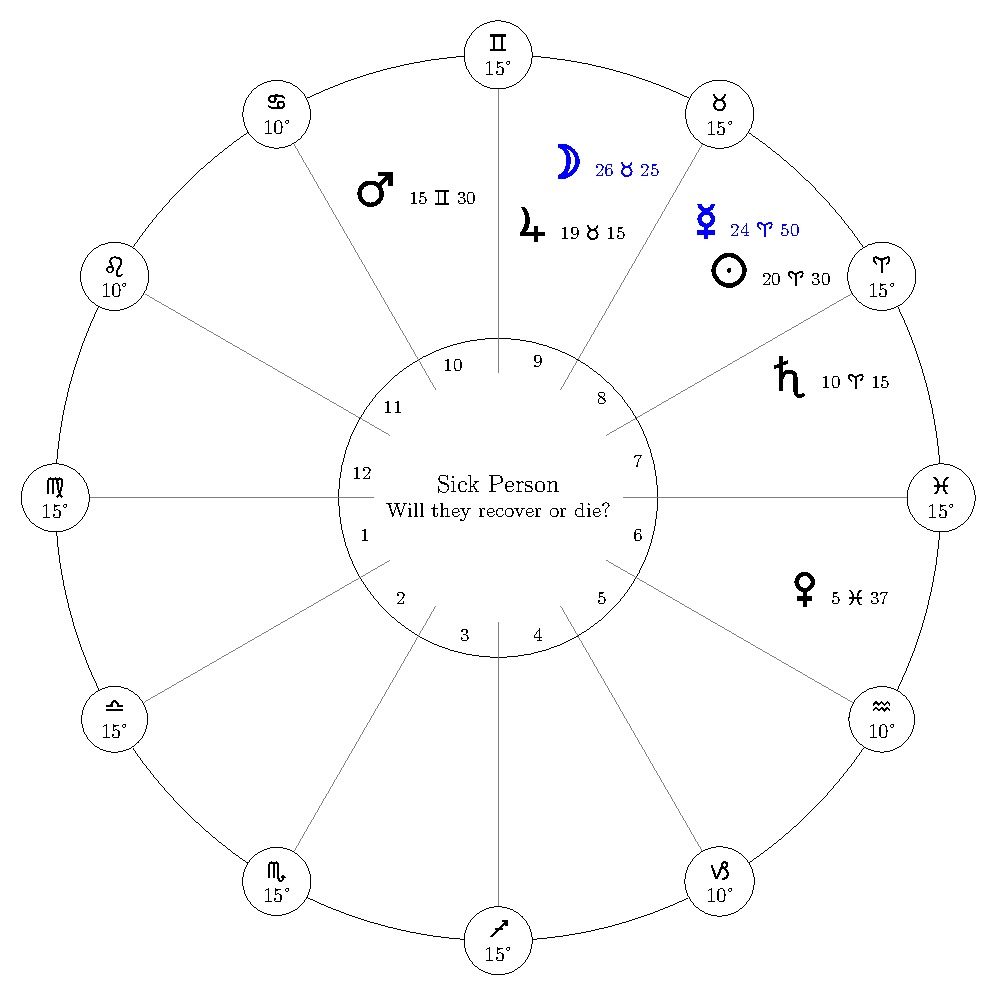
\includegraphics[width=0.9\textwidth]{charts/21-chart-sickness}} \\
\vspace{-0.2cm}
\end{center}
\end{columns}
\footnotetext[1]{He can only apply to \Saturn\ and he is already separated from him.}
\end{frame}
% ------------------------------------------------------------
\begin{frame}[t]{Example Chart: Sickness Continued}

After examining the \Moon\ committing her dispostion, Masha'allah then looks at L1 as sharing in the matter and finds it confirms what the \Moon\ signified:

\textbf{\Mercury\ in \Aries\ Void of Course} $\Rightarrow$ \Taurus \\
$\Rightarrow$ \Sextile\ \Venus\ \Pisces\ who receives him from \Taurus \\
\Venus\ $\Rightarrow$ \Trine\ \Jupiter\ in \Taurus\, MR by domicile \\
And again, \Jupiter\ is the end of the disposition chain, supporting what the \Moon\ indicated.
\vspace{0.2cm}

\Jupiter, a benefic, as the final arbiter of the disposition promises "health and quiet" and the end of the illness after a prolonged period (due to the VOC's) but we are told that from the time of \Venus\ accepting the \Moon's disposition to her joining with \Jupiter, the person would have gradually strengthened, with the illness leaving him completely once \Venus\ separates from \Jupiter\ by one minute.

\end{frame}
% -------------------------------------------------------------------------
\begin{frame}[t]{Example Chart: Sickness (Alternative Scenarios)}
One odd thing here, how does \Venus\ join with \Jupiter's \Sextile\ at 19 \Pisces\ before it joins with \Mars's \Square\ at 15 \Pisces? Even assuming he took the aspect moieties into account, \Venus\ would have been within moiety of \Mars\ \Square\ at 7.5° \Pisces (15 - (7+8)/2)) which is less than \Jupiter's \Sextile\ moiety of 11 \Pisces (19-(9+7)/2). 

\vspace{0.3cm}
Masha'allah does list the \Mars\ connection as an alternative scenario, saying such a connection would have meant death for the querent as \Mars's is L8 and does not receive \Venus. So perhaps, the \Moon\ $\rightarrow$ \Venus\ $\rightarrow$ \Jupiter\ connections are also simply to illustrate a point.

He goes on to warn that the \Sun, if not L1, destroys by combustion if he does not receive the planet, and this also applies to his \Square\ or \Opposition. [JH]p23.\footnotemark[1]

\footnotetext[1]{I've seen this before as a planet being protected from combustion if he's in his own signs; here, they have be in the \Sun's signs (\Leo\ or \Aries) where the \Sun\ will receive them and so protect them.}
\end{frame}